\begin{figure*}[!htb]
	\centering
		%\hline
		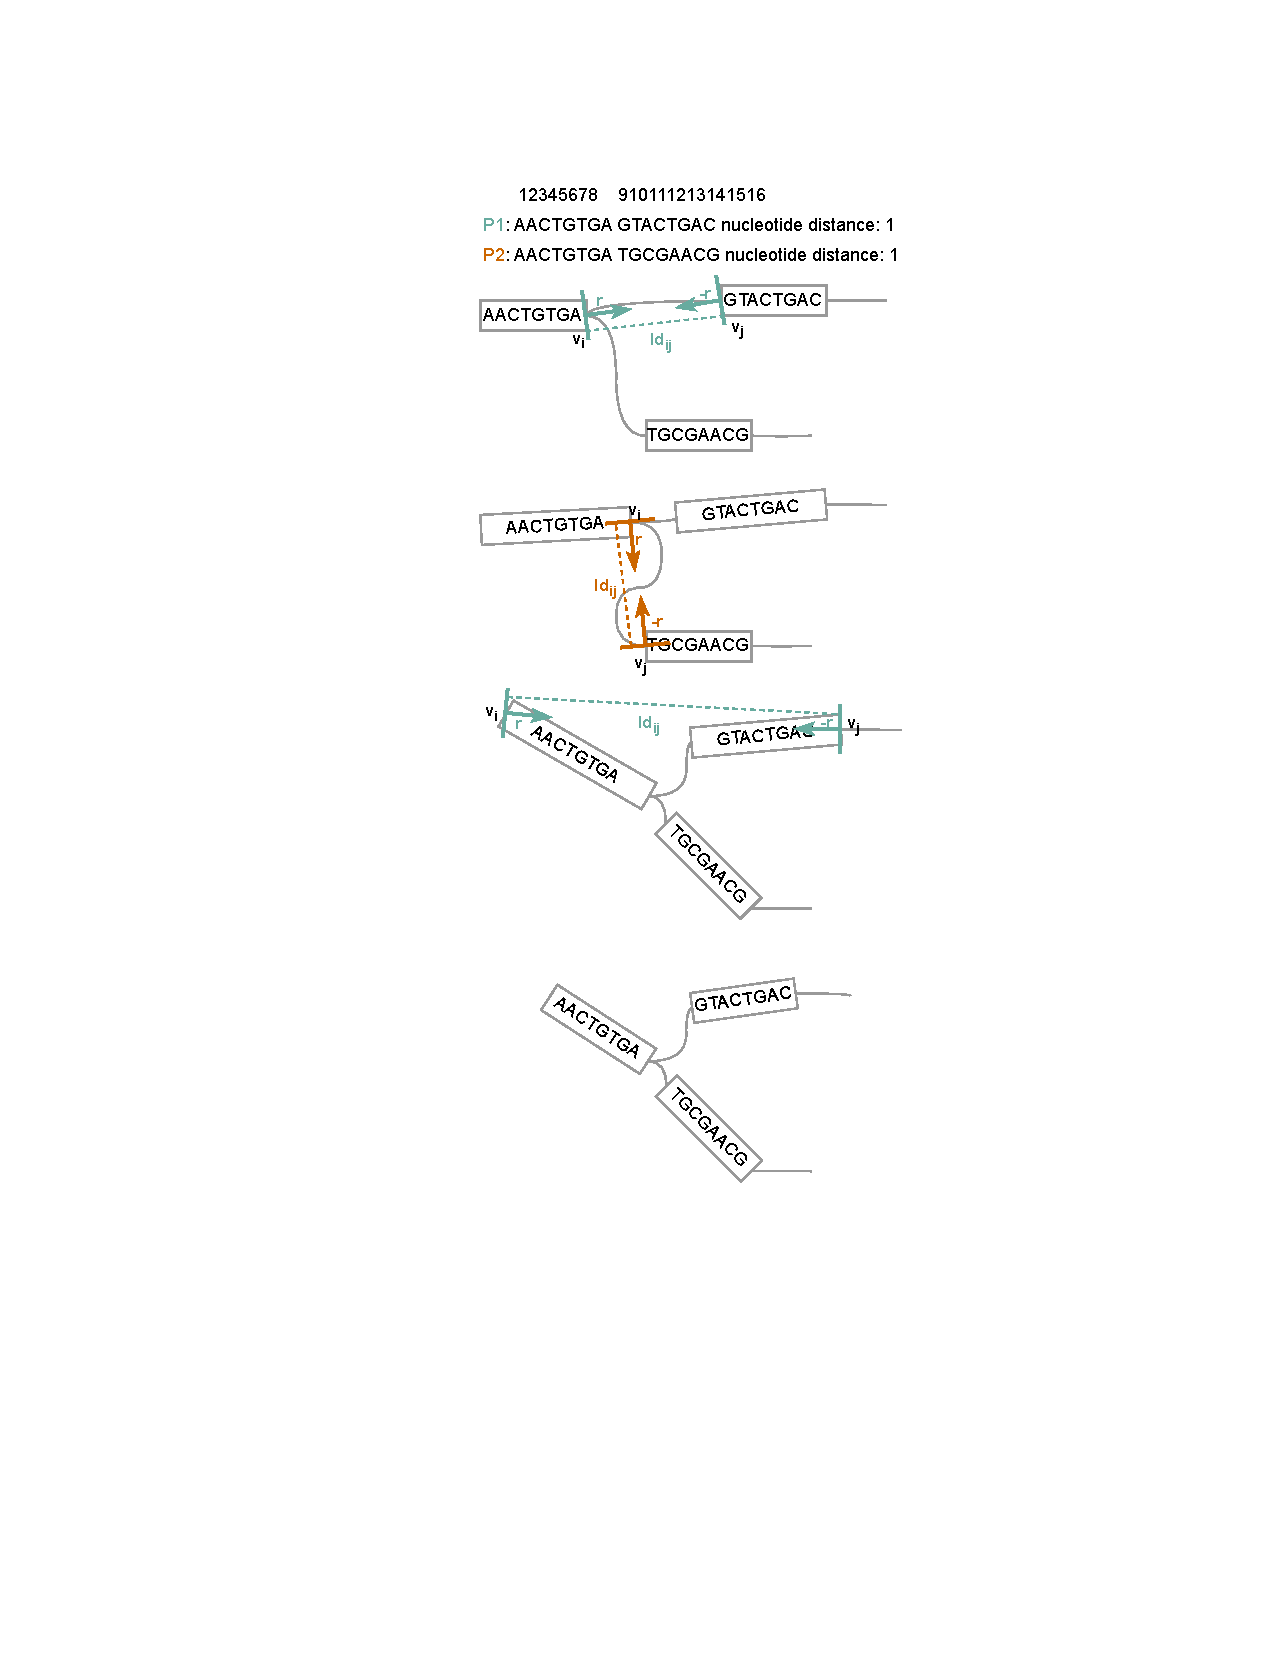
\includegraphics[width=\linewidth, trim=0cm 8cm 0cm 0cm, clip]{fig/sketches/PG-SGD.drawio.pdf}
	\caption{
		2D PG-SGD update operation sketches. \textbf{(a)} The path information of the graph which is going to be updated. Top: Path positions. Bottom: Path names with path sequences and the nucleotide distance between two consecutive nodes. \textbf{(b-e)} $v_i$ and $v_j$ is the current pair of nodes to update. $ld_{ij}$ is the current layout distance. $r,-r$ is the current size of the update. \textbf{(b)} Initial graph layout highlighting the future update of the two nodes of path \textit{P1}. \textbf{(c)} The graph layout after the first update. The nodes appear longer now, because we updated at the end of the nodes. Highlighted is the future update of the two nodes of path \textit{P2}. \textbf{(d)} The graph layout after the second update. Highlighted is the future update of the two nodes of \textit{P1}. \textbf{(e)} Final graph layout after three updates using the 2D PG-SGD.  \\
		\FIXME{PROVIDE SEVERAL NICE FIGURES SO WE CAN REARRANGE STUFF INTO SUBFIGURES.}
	}
	\label{fig:sketches}
\end{figure*}